\section{电流的磁场}\label{sec:10-4}

人们早就发现带电体和磁体有某些相似的性质。
例如,对于带电体,同种电荷互相推斥,异种电荷互相吸引;
对于磁体,同名磁极互相推斥,异名磁极互相吸引。
带电体和磁体的这些相似,是一种巧合吗了?
科学家早就猜想电和磁之间可能有某种关系,并一次又一次地通过实验来寻找这种关系。
1820 年,丹麦的奥斯特在静止的磁针上方拉一根与磁针平行的导线,给导线通电时,
磁针立刻偏转一个角度(图 \ref{fig:10-16}),切断电流时,磁针又回到原来位置。
奥斯特的实验表明:通电导线的周围和磁铁的周围一样,存在着磁场。
正是电流产生的磁场作用于磁针,使磁针发生了偏转。

\begin{figure}[htbp]
    \centering
    \begin{minipage}{7cm}
    \centering
    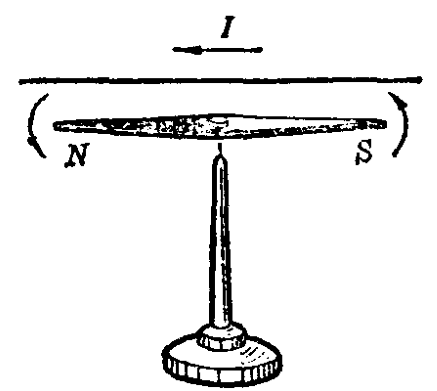
\includegraphics[width=5cm]{../pic/czwl2-ch10-16}
    \caption{奥斯特实验}\label{fig:10-16}
    \end{minipage}
    \qquad
    \begin{minipage}{7cm}
    \centering
    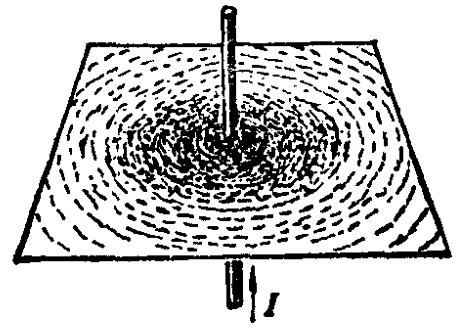
\includegraphics[width=6cm]{../pic/czwl2-ch10-17}
    \caption{直线电流的磁场}\label{fig:10-17}
    \end{minipage}
\end{figure}

既然电流的周围存在着磁场,那么电流周围的磁场是怎样的呢?我们仍然可以利用铁屑来观察。

取一根直导线,垂直穿过一块硬纸板。在纸板上均匀地撒上一层铁屑,给导线通电,轻敲纸板,
铁屑就在导线周围排成一圈一圈的同心圆(图 \ref{fig:10-17})。
上下移动纸板,在不同的位置重做上面的实验,铁屑的排列情况不变,
这表明直线电流周围的磁力线是一些以导线上各点为圆心的同心圆,这些同心圆都在跟导线垂直的平面上。

\begin{figure}[H]%[htbp]
    \centering
    \begin{minipage}{7cm}
    \centering
    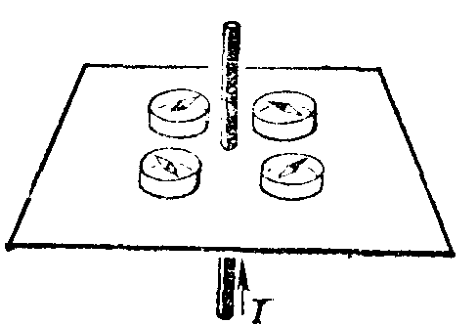
\includegraphics[width=6cm]{../pic/czwl2-ch10-18}
    \caption{}\label{fig:10-18}
    \end{minipage}
    \qquad
    \begin{minipage}{7cm}
    \centering
    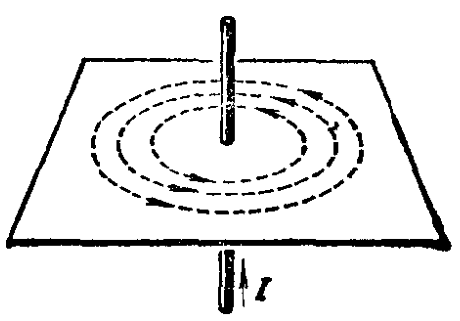
\includegraphics[width=6cm]{../pic/czwl2-ch10-19}
    \caption{}\label{fig:10-19}
    \end{minipage}
\end{figure}

\begin{wrapfigure}[14]{r}{5cm}
    \centering
    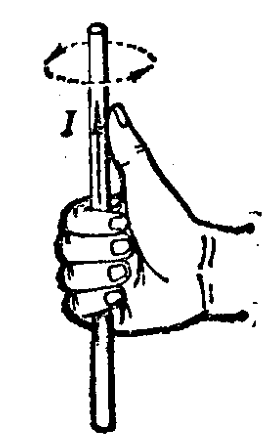
\includegraphics[width=4cm]{../pic/czwl2-ch10-20}
    \caption{安培定则(一)}\label{fig:10-20}
\end{wrapfigure}

直线电流的磁力线方向,可以用小磁针来确定。
照图 \ref{fig:10-18} 那样,在纸板上放几个小磁针,
导线通电时小针北极所指的方向就是磁针所在处的磁力线的方向(图 \ref{fig:10-19})。
如果改变导线中电流的方向,小磁针的北极立刻转向相反的方向。


直线电流周围的磁力线的方向跟电流的方向之间的关系可以用安培定则
\footnote{安培定则在有些书上也叫右手螺旋定则。}来判定。照图 \ref{fig:10-20} 那样,
\CJKunderwave{用右手握住导线,让大拇指所指的方向跟电流的方向一致,那么弯曲的四指所指的方向就是磁力线的环绕方向}。

把导线绕成螺线管,通电以后,它周围的小磁针也发生偏转,这表明通电螺线管周围也存在着磁场。
用铁屑来做实验,可以看到,通电螺线管周围的磁力线跟条形磁铁的磁力线相似(图 \ref{fig:10-21})。

把小磁针靠近通电螺线管可以看到,螺线管的一端跟磁针的北极相吸引,另一端跟磁针的南极相吸引。
这表明通电螺线管也有两个磁极。


\begin{figure}[htbp]
    \centering
    \begin{minipage}{7cm}
    \centering
    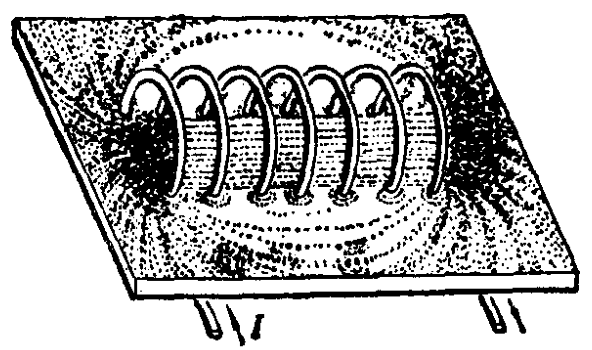
\includegraphics[width=6cm]{../pic/czwl2-ch10-21}
    \caption{通电螺线管的磁场}\label{fig:10-21}
    \end{minipage}
    \qquad
    \begin{minipage}{7cm}
    \centering
    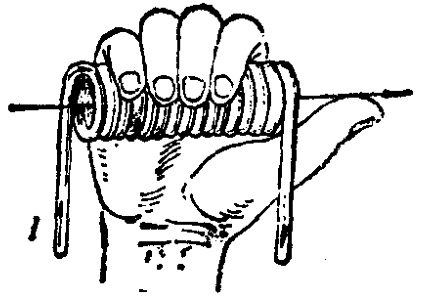
\includegraphics[width=6cm]{../pic/czwl2-ch10-22}
    \caption{安培定则(二)}\label{fig:10-22}
    \end{minipage}
\end{figure}

当电流方向改变时,螺线管的南北极正好对调。
可见,通电螺线管两端的磁极性质跟电流方向有关系,它们之间的关系也可以用安培定则来判定。
照图 \ref{fig:10-22} 那样,
\CJKunderwave{用右手握住螺线管,让弯曲的四指所指的方向跟电流的方向一致,那么大拇指所指的那端就星也螺线管的北极}。


\newpage

\lianxi

(1) 已知通电直导线周围的磁力线方向如图 \ref{fig:10-23} 所示,你能说出导线中的电流方向吗? 把它标在图上。

\begin{figure}[htbp]
    \centering
    \begin{minipage}{7cm}
    \centering
    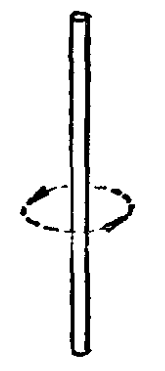
\includegraphics[width=2cm]{../pic/czwl2-ch10-23}
    \caption{}\label{fig:10-23}
    \end{minipage}
    \qquad
    \begin{minipage}{7cm}
    \centering
    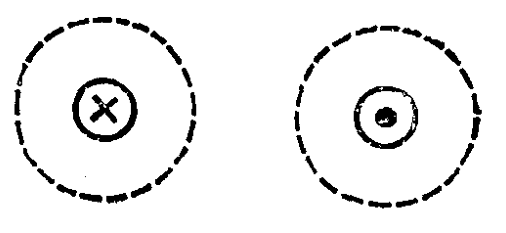
\includegraphics[width=6cm]{../pic/czwl2-ch10-24}
    \caption{}\label{fig:10-24}
    \end{minipage}
\end{figure}


(2) 在图 \ref{fig:10-24} 中,里而的小圆圈表示通电导线的横截面。
小圆圈里面画一个 “×” 号表示电流方向是垂直纸面从纸外进入纸里;
画一个圆点表示电流方向是垂直纸面从纸里出来。
外面的大圆圈表示磁力线,试根据电流方向标出磁力线的方向。

(3) 在图 \ref{fig:10-25} 中,标出通电螺线管的 $N$ 极和 $S$ 极。

\begin{figure}[htbp]
    \centering
    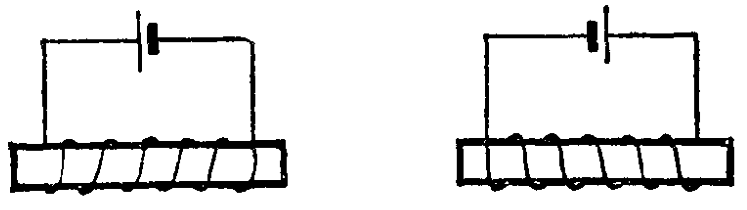
\includegraphics[width=0.6\textwidth]{../pic/czwl2-ch10-25}
    \caption{}\label{fig:10-25}
\end{figure}

(4) 在图 \ref{fig:10-26} 中,标出通电螺线管的电流方向。

\begin{figure}[htbp]
    \centering
    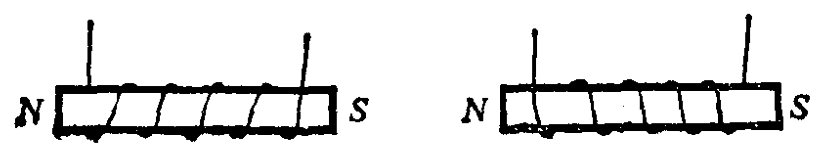
\includegraphics[width=0.6\textwidth]{../pic/czwl2-ch10-26}
    \caption{}\label{fig:10-26}
\end{figure}


\section*{小实验}

奥斯特发现电流的磁效应是很不容易的。
但是在我们知道这个发现以后,却很容易自己来观察这个现象。
下面的小实验是每个同学都可以自己动手做的。

把一根已磁化的针插在一片软木上,再把它水平地放在一盆水中,让它浮在水面上,
静止时磁针将指向南北方向(图 \ref{fig:10-27})。 然后,在针的上面平行地拉一条导线,
当把导线的两端连在电池的两极上时(注意通电时间不可过长), 磁针就偏转一个角度。
在接通电路前,你能判断出通电后磁针向哪个方向偏转吗?

\begin{figure}[H]%[htbp]
    \centering
    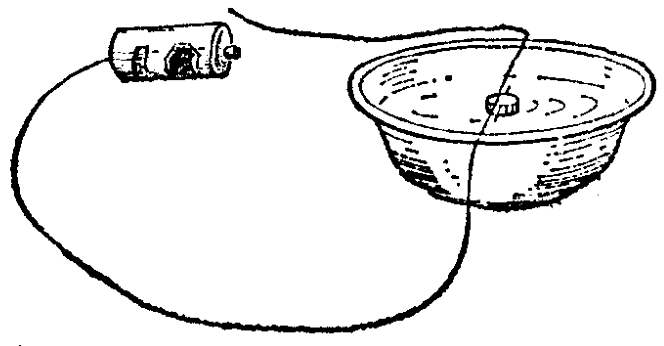
\includegraphics[width=0.6\textwidth]{../pic/czwl2-ch10-27}
    \caption{}\label{fig:10-27}
\end{figure}

